\documentclass[12pt]{article}
\usepackage{amsmath}
\usepackage{graphicx}
\usepackage{hyperref}
\usepackage{listings}
\usepackage{color}
\usepackage{pythonhighlight}

\title{Operating System Course Report - First Half of the Semester}
\author{A class}
\date{\today}

\begin{document}

\maketitle
\newpage

\tableofcontents
\newpage

\section{Introduction}
This report summarizes the topics covered during the first half of the Operating System course. It includes theoretical concepts, practical implementations, and assignments. The course focuses on the fundamentals of operating systems, including system architecture, process management, CPU scheduling, and deadlock handling.

\section{Course Overview}
\subsection{Objectives}
The main objectives of this course are:
\begin{itemize}
    \item To understand the basic components and architecture of a computer system.
    \item To learn process management, scheduling, and inter-process communication.
    \item To explore file systems, input/output management, and virtualization.
    \item To study the prevention and handling of deadlocks in operating systems.
\end{itemize}

\subsection{Course Structure}
The course is divided into two halves. This report focuses on the first half, which covers:
\begin{itemize}
    \item Basic Concepts and Components of Computer Systems
    \item System Performance and Metrics
    \item System Architecture of Computer Systems
    \item Process Description and Control
    \item Scheduling Algorithms
    \item Process Creation and Termination
    \item Introduction to Threads
    \item File Systems
    \item Input and Output Management
    \item Deadlock Introduction and Prevention
    \item User Interface Management
    \item Virtualization in Operating Systems
\end{itemize}

\section{Topics Covered}

\subsection{Basic Concepts and Components of Computer Systems}
This section explains the fundamental components that make up a computer system, including the CPU, memory, storage, and input/output devices.

\subsection{System Performance and Metrics}
This section introduces various system performance metrics used to measure the efficiency of a computer system, including throughput, response time, and utilization.

\subsection{System Architecture of Computer Systems}
Describes the architecture of modern computer systems, focusing on the interaction between hardware and the operating system.

\subsection{Process Description and Control}
Processes are a central concept in operating systems. This section covers:
\begin{itemize}
    \item Process states and state transitions
    \item Process control block (PCB)
    \item Context switching
\end{itemize}

\subsection{Scheduling Algorithms}
This section covers:
\begin{itemize}
    \item First-Come, First-Served (FCFS)
    \item Shortest Job Next (SJN)
    \item Round Robin (RR)
\end{itemize}
It explains how these algorithms are used to allocate CPU time to processes.

\subsection{Process Creation and Termination}
\subsubsection{\textit{Process Creation}}
(Isi materi disini)

\subsubsection{Siapa yang Membuat Proses}
(Isi materi disini)

\subsubsection{Proses \textit{Termination}}
\begin{itemize}
    \item Definisi Proses \textit{Termination}
     (isi materi disini)

    \item Jenis-jenis \textit{Termination}
    (Isi materi disini)

    \item Apa yang Terjadi Setelah \textit{Termination}
    

    Setelah proses dibuat, proses tersebut mulai berjalan dan melakukan apa 
    pun tugasnya. Namun, tidak ada yang bertahan selamanya, bahkan tidak proses. 
    Cepat atau lambat proses baru akan berhenti, biasanya karena salah satu kondisi 
    berikut :

    \begin{enumerate}
        \item Normal \textit{Exit} (voluntary)
        \item Error \textit{Exit} (voluntary)
        \item Fatal \textit{Exit} (involuntary)
        \item \textit{Killed by another process (involuntary)}
    \end{enumerate}

    Sebagian besar proses berhenti karena mereka telah menyelesaikan 
    tugasnya. Saat menjadi compiler telah mengkompilasi program yang diberikan 
    padanya, kompilator mengeksekusi panggilan sistem untuk memberitahu sistem 
    operasi yang sudah selesai. Panggilan ini keluar di UNIX dan \textit{ExitProcess} di 
    Windows. Program berorientasi layar juga mendukung penghentian sukarela. 
    Kata prosesor, browser Internet, dan program serupa selalu memiliki ikon atau 
    menu item yang dapat diklik pengguna untuk memberi tahu proses untuk 
    menghapus file sementara yang dimilikinya buka lalu akhiri

    Alasan kedua untuk penghentian adalah karena proses tersebut 
    menemukan kesalahan fatal.

    Alasan ketiga penghentian adalah kesalahan yang disebabkan oleh 
    proses, seringkali karena bug program. Contohnya termasuk menjalankan 
    instruksi ilegal, referensi memori yang tidak ada, atau membaginya dengan nol. 
    Di beberapa sistem (misalnya, UNIX), sebuah proses dapat memberi tahu sistem 
    operasi bahwa ia ingin menangani kesalahan tertentu itu sendiri, di mana kasus 
    proses ini ditandai (terputus) bukannya dihentikan ketika salah satu kesalahan 
    terjadi.

    Alasan keempat suatu proses mungkin berhenti adalah bahwa proses 
    tersebut menjalankan panggilan sistem yang memberi tahu sistem operasi untuk 
    menghentikan beberapa proses lain. Di UNIX panggilan ini adalah membunuh. 
    Fungsi Win32 yang sesuai adalah \textit{TerminateProcess}.

    Setelah sebuah proses dihentikan di sistem operasi, ada beberapa hal yang terjadi di balik layar untuk memastikan semuanya berjalan dengan lancar. Mari kita bahas ini dengan cara yang santai.
    \begin{enumerate}
        \item Pembebasan Sumber Daya
        

        Setiap proses yang berjalan di komputer 
        menggunakan berbagai sumber daya, seperti 
        memori, CPU, \textit{file}, dan perangkat keras lainnya. 
        Ketika proses tersebut dihentikan, semua sumber daya 
        yang telah dipinjam oleh proses itu harus dikembalikan ke 
        sistem agar bisa digunakan oleh proses lain. 
        \item Tanda Bahwa Proses Selesai
        

        Ketika sebuah proses dihentikan, OS akan menandai bahwa 
        proses tersebut sudah selesai. Ini penting agar OS tidak 
        mencoba menjalankan kembali proses yang sudah selesai. 
        Selain itu, informasi tentang bagaimana proses itu berakhir 
        (apakah sukses atau terjadi error) disimpan oleh OS.

        \textit{Exit} Status: Setelah proses berhenti, biasanya ada 
        semacam kode yang dikembalikan untuk menunjukkan 
        apakah proses itu berhasil atau ada masalah. Ini disebut 
        \textit{exit} status. Jika proses berjalan lancar, \textit{exit} status-nya 
        mungkin 0(nol). Kalau ada masalah, \textit{exit} status-nya bisa berupa 
        angka lain yang menunjukkan \textit{error}.

        \item Membersihkan Proses dari Daftar
        

        Sistem operasi memiliki daftar semua proses yang sedang 
        berjalan. Ketika sebuah proses selesai, OS akan menghapus 
        proses itu dari daftar. Ini seperti menandai bahwa pekerjaan 
        selesai sehingga OS tidak lagi memperhitungkan proses 
        tersebut.

        \item  Menginformasikan Proses Lain
        

        Kadang-kadang, ada proses lain yang bergantung pada proses 
        yang baru saja dihentikan. OS akan memberitahukan proses-proses 
        tersebut bahwa proses yang mereka tunggu sudah selesai. 
        Ini memungkinkan proses lain untuk melanjutkan tugasnya.

        \item  \textit{Logging} atau Pencatatan
        

        Terakhir, beberapa sistem operasi akan mencatat bahwa 
        sebuah proses telah dihentikan dalam \textit{log} sistem. Ini 
        seperti mencatat dalam buku harian tentang apa yang telah 
        terjadi. Informasi ini bisa berguna jika ada masalah atau
        jika kamu ingin melihat apa yang telah dilakukan komputer 
        di masa lalu. 
    \end{enumerate}
\end{itemize}
\begin{thebibliography}{99}
    \bibitem{}
    Octaviano, A., Junianto, M. B. S., \& Saprudin, S. (2022). SISTEM OPERASI.
    \bibitem{}
    Pangera, A. A., \& Ariyus, D. (2005). Sistem Operasi. Penerbit Andi.
\end{thebibliography}

\subsection{Introduction to Threads}
This section introduces the concept of threads and their relation to processes, covering:
\begin{itemize}
    \item Single-threaded vs. multi-threaded processes
    \item Benefits of multithreading
\end{itemize}

\begin{figure}[h]
    \centering
    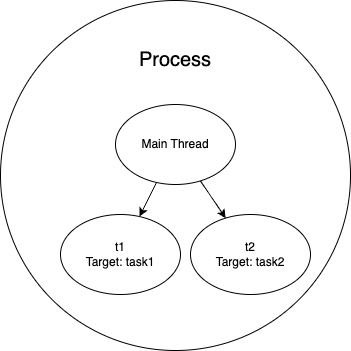
\includegraphics[width=0.5\textwidth]{D:/Repo Sisop/os_report_mid2024/a_class/asset/example.png}  % Sesuaikan nama file dan ukurannya
    \caption{Ini adalah gambar contoh dari multithreading.}
    \label{fig:contoh_gambar}
\end{figure}

Seperti yang terlihat pada Gambar \ref{fig:contoh_gambar}, inilah cara menambahkan gambar dengan keterangan.

\subsection{File Systems}
File systems provide a way for the operating system to store, retrieve, and manage data. This section explains:
\begin{itemize}
    \item File system structure
    \item File access methods
    \item Directory management
\end{itemize}

\subsection{Input and Output Management}
Input and output management is key for handling the interaction between the system and external devices. This section includes:
\begin{itemize}
    \item Device drivers
    \item I/O scheduling
\end{itemize}

\subsection{Deadlock Introduction and Prevention}
Explores the concept of deadlocks and methods for preventing them:
\begin{itemize}
    \item Deadlock conditions
    \item Deadlock prevention techniques
\end{itemize}

\subsection{User Interface Management}
This section discusses the role of the operating system in managing the user interface. Topics covered include:
\begin{itemize}
    \item Graphical User Interface (GUI)
    \item Command-Line Interface (CLI)
    \item Interaction between the user and the operating system
\end{itemize}

\subsection{Virtualization in Operating Systems}
Virtualization allows multiple operating systems to run concurrently on a single physical machine. This section explores:
\begin{itemize}
    \item Concept of virtualization
    \item Hypervisors and their types
    \item Benefits of virtualization in modern computing
\end{itemize}

\section{Assignments and Practical Work}
\subsection{Assignment 1: Process Scheduling}
Students were tasked with implementing various process scheduling algorithms (e.g., FCFS, SJN, and RR) and comparing their performance under different conditions.
\subsubsection{Group 1}
\begin{python}
    class Process:
    def __init__(self, pid, arrival_time, burst_time):
        self.pid = pid
        self.arrival_time = arrival_time
        self.burst_time = burst_time
        self.completion_time = 0
        self.turnaround_time = 0
        self.waiting_time = 0
\end{python}

\begin{table}[htbp] % Optional: For floating position
    \centering
    \begin{tabular}{|c|c|c|} % Defines number of columns and alignment (c = center, l = left, r = right). '|' creates vertical lines.
    \hline
    Header 1 & Header 2 & Header 3 \\ % Column headers
    \hline
    Row 1, Column 1 & Row 1, Column 2 & Row 1, Column 3 \\ % First row of data
    \hline
    Row 2, Column 1 & Row 2, Column 2 & Row 2, Column 3 \\ % Second row of data
    \hline
    \end{tabular}
    \caption{Your table caption} % Optional: For adding a caption
    \label{tab:your_label} % Optional: For cross-referencing the table
\end{table}
\subsection{Assignment 2: Deadlock Handling}
In this assignment, students were asked to simulate different deadlock scenarios and explore various prevention methods.

\subsection{Assignment 3: Multithreading and Amdahl's Law}
This assignment involved designing a multithreading scenario to solve a computationally intensive problem. Students then applied **Amdahl's Law** to calculate the theoretical speedup of the program as the number of threads increased.

\subsection{Assignment 4: Simple Command-Line Interface (CLI) for User Interface Management}
Students were tasked with creating a simple **CLI** for user interface management. The CLI should support basic commands such as file manipulation (creating, listing, and deleting files), process management, and system status reporting.
\subsubsection {Group 6}
Tuliskan implementasi CLI sederhana yang dapat melakukan perintah berikut:

\subsubsection{Group 6}

\textbf{Soal:}

Buatlah \textit{Simple CLI} menggunakan Python, lalu lakukan serangkaian operasi berikut dan catat hasilnya:

    \begin{enumerate}
        \item Buat sebuah berkas bernama \texttt{laporan.txt}.
        \item Tampilkan daftar berkas dalam direktori saat ini.
        \item Tampilkan status sistem.
        \item Tampilkan daftar proses yang sedang berjalan.
        \item Hapus berkas \texttt{laporan.txt} yang telah dibuat sebelumnya.
        \item Tampilkan kembali daftar berkas dalam direktori saat ini.
    \end{enumerate}

Berikan tangkapan layar atau salin keluaran dari setiap langkah di atas.

\textbf{Jawaban:}

\begin{lstlisting}
import os
import psutil
import datetime

def create_file(filename):
    with open(filename, 'w') as f:
        f.write("This is a new file.")
    return f"File '{filename}' created successfully."

def list_files():
    files = os.listdir('.')
    return "\n".join(files)

def delete_file(filename):
    if os.path.exists(filename):
        os.remove(filename)
        return f"File '{filename}' deleted successfully."
    else:
        return f"File '{filename}' not found."

def list_processes():
    processes = []
    for proc in psutil.process_iter(['pid', 'name']):
        processes.append(f"{proc.info['pid']}: {proc.info['name']}")
    return "\n".join(processes[:10])  # Limiting to first 10 for brevity

def system_status():
    cpu_percent = psutil.cpu_percent()
    memory = psutil.virtual_memory()
    disk = psutil.disk_usage('C:\\')  # Ganti '/' dengan 'C:\\'
    
    return f"CPU Usage: {cpu_percent}%\nMemory Usage: {memory.percent}%\nDisk Usage: {disk.percent}%"

def main():
    print("Welcome to the Simple CLI Simulator!")
    print("Type 'help' for a list of commands.")
    
    while True:
        command = input(">>> ").strip().lower()
        
        if command == "exit":
            print("Goodbye!")
            break
        elif command == "help":
            print("Available commands:")
            print("  create <filename> - Create a new file")
            print("  list - List files in the current directory")
            print("  delete <filename> - Delete a file")
            print("  processes - List running processes")
            print("  status - Show system status")
            print("  exit - Exit the CLI")
        elif command.startswith("create "):
            filename = command.split(" ", 1)[1]
            print(create_file(filename))
        elif command == "list":
            print(list_files())
        elif command.startswith("delete "):
            filename = command.split(" ", 1)[1]
            print(delete_file(filename))
        elif command == "processes":
            print(list_processes())
        elif command == "status":
            print(system_status())
        else:
            print("Unknown command. Type 'help' for a list of commands.")

if _name_ == "_main_":
    main()
\end{lstlisting}

\textbf{\textit{Output:}}

\begin{figure}[h]
    \centering
    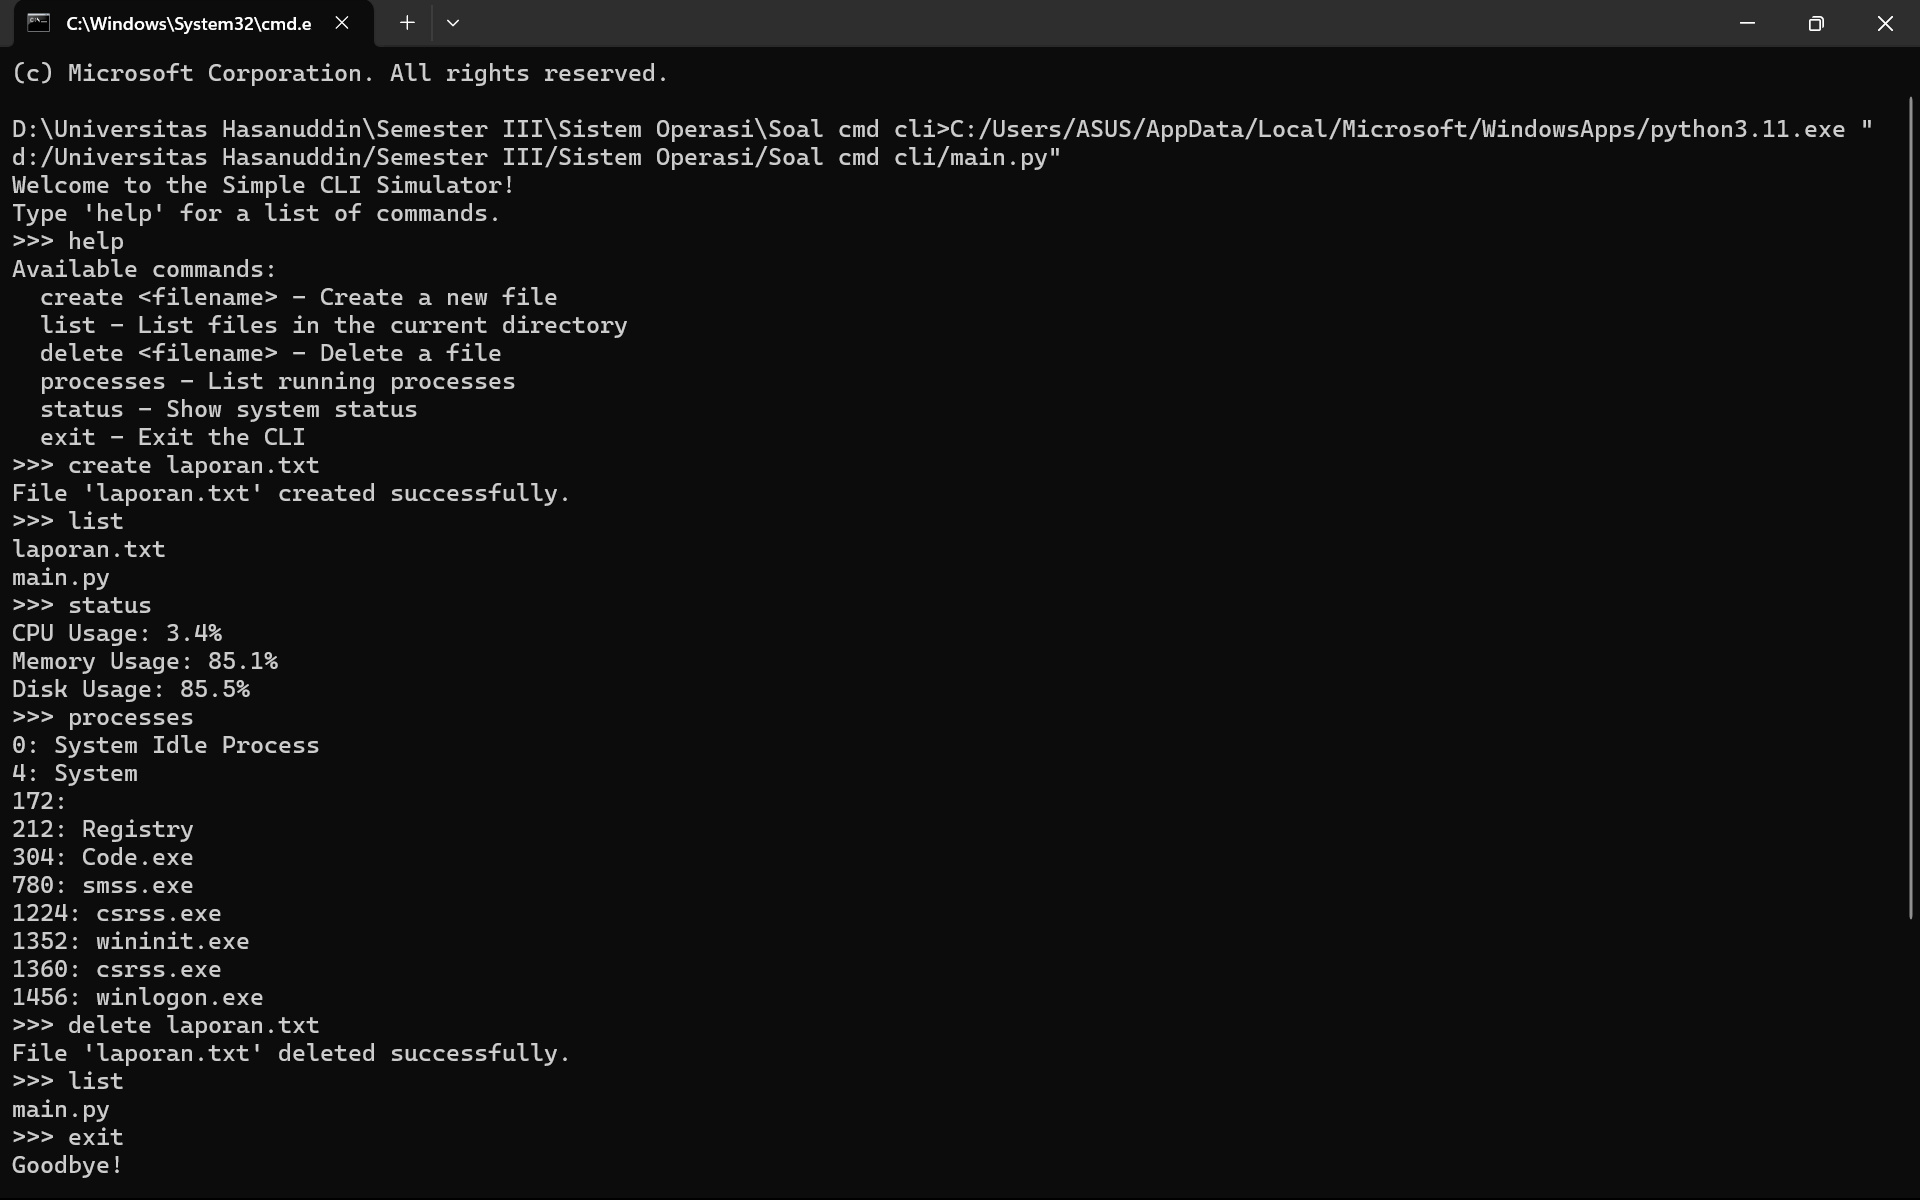
\includegraphics[width=1\textwidth]{D:/Repo Sisop/os_report_mid2024/a_class/asset/Screenshot 2024-10-03 114321.png}
    \caption{\textit{Output} Kode}
\end{figure}


\subsection{Assignment 5: File System Access}
In this assignment, students implemented file system access routines, including:
\begin{itemize}
    \item File creation and deletion
    \item Reading from and writing to files
    \item Navigating directories and managing file permissions
\end{itemize}


\section{Conclusion}
The first half of the course introduced core operating system concepts, including process management, scheduling, multithreading, and file system access. These topics provided a foundation for more advanced topics to be covered in the second half of the course.

\end{document}